\documentclass{article}
\PassOptionsToPackage{numbers,sort&compress}{natbib}

% "preprint" = non-anonymous (group members are listed), no line numbers.
\usepackage[preprint]{neurips_2026}

\usepackage[utf8]{inputenc}
\usepackage[T1]{fontenc}
\usepackage{hyperref}
\usepackage{url}
\usepackage{booktabs}
\usepackage{amsfonts,amsmath}
\usepackage{nicefrac}
\usepackage{microtype}
\usepackage{xcolor}
\usepackage{graphicx}
\usepackage{tikz}
\usepackage{wrapfig}
\usepackage{tabularx}
\usepackage{enumitem}
\usepackage{listings}
\usepackage{float}

% Shared TikZ styles for all Gloss proposal figures.
% Loaded by main.tex and by the standalone wrappers in ../../tools/.
\usetikzlibrary{arrows.meta,positioning,fit,backgrounds,calc,shapes.geometric}

\definecolor{glpurple}{HTML}{6D4AFF}
\definecolor{glblue}{HTML}{2F7CF6}
\definecolor{glgreen}{HTML}{1F9D6B}
\definecolor{glorange}{HTML}{E8871E}
\definecolor{glred}{HTML}{D64545}
\definecolor{glgray}{HTML}{6B7280}
\definecolor{glink}{HTML}{1F2937}

\tikzset{
  gl/.style={font=\sffamily\scriptsize, >=Stealth, line width=0.5pt, text=glink},
  box/.style={draw, rounded corners=2pt, align=center, inner sep=2.5pt},
  gstep/.style={box, fill=glpurple!10, draw=glpurple, minimum width=1.78cm, minimum height=0.95cm},
  ctx/.style={box, fill=glblue!8, draw=glblue, minimum width=3.15cm, minimum height=0.95cm},
  kern/.style={box, fill=glgray!10, draw=glgray, minimum width=2.4cm, minimum height=0.75cm},
  adp/.style={box, fill=glgreen!9, draw=glgreen!80!black, minimum width=2.1cm, minimum height=0.8cm},
  chip/.style={draw=glorange, fill=glorange!12, rounded corners=5pt, inner sep=2pt,
               font=\sffamily\tiny\bfseries, minimum height=0.38cm, minimum width=1.2cm},
  frame/.style={draw=#1, rounded corners=4pt, dashed, inner sep=4pt},
  framelabel/.style={font=\sffamily\tiny\bfseries, text=#1, fill=white, inner sep=1pt},
  flow/.style={->, draw=glink},
  io/.style={box, fill=white, draw=glink, minimum width=2.0cm, minimum height=1.3cm},
}


% One place to rename the system (e.g. "Gloss Agent").
\newcommand{\sysname}{GlossX}
\newcommand{\gloss}{Gloss}

\makeatletter
\renewcommand{\@noticestring}{Course project proposal (Agentic AI), October 2026.}
\makeatother

\setlist{leftmargin=1.2em, itemsep=1pt, topsep=2pt, parsep=0pt}
\hypersetup{colorlinks=true, linkcolor=glpurple, citecolor=glblue, urlcolor=glblue}
\lstset{basicstyle=\ttfamily\scriptsize, columns=fullflexible, frame=single,
        rulecolor=\color{glgray!60}, breaklines=true}

\title{\sysname: An Open, Plugin-Native Agent Harness\\for Research and Learning}

% Group members (contact member marked with a footnote).
\author{%
  Cai Jiechao\thanks{Contact member: \texttt{u3679152@connect.hku.hk}} \\ UID: u3679152
  \And
  Cai Zhuorui \\ UID: u3679195
  \And
  Sun Zhiwei \\ UID: u3679115
  \And
  Zhang Guanyi \\ UID: u3679381
  \AND
  The University of Hong Kong
}

\begin{document}
\maketitle

\begin{abstract}
Research and study are long, tool-heavy activities---finding, reading, comparing, verifying, reproducing and learning---yet today's agents specialise elsewhere: coding agents (Claude Code, Codex), office agents (WorkBuddy) and personal assistants (Meta Muse, OpenAI Dots). We propose \sysname{}, which evolves \gloss{}, our released open-source paper reader, into an \emph{open, plugin-native agent harness for research and learning}. A small kernel exposes one \emph{Capability ABI} through which document sources, tools, sub-agents, loops, deciders, memories, Agent Skills, MCP servers and coding agents are all mounted as plugins. A core agent routes each request to a workflow, plans a typed step graph, executes sub-agents in parallel, verifies every claim against source spans and reflects until an explicit stop condition holds, while a tiered context manager passes pointers instead of text. We will evaluate on PaperArena, AutoResearchBench, LitSearch, ScholarQABench, QASPER, SciFact, PaperBench Code-Dev and TutorBench, plus harness-level tests of routing, robustness, cost and extensibility.
\end{abstract}

% =====================================================================
\section{Project Objective}
\label{sec:objective}

\textbf{What \gloss{} is today.} \gloss{}~\cite{gloss2026} is an open-source, self-hosted AI companion for reading research papers that we built and released (v1.0.2, July 2026; Windows desktop app and npm package; CI on Linux and Windows). A FastAPI backend serves a React/PDF.js reader with a real text layer and drives four interchangeable LLM providers: the local Claude Code~\cite{claudecode} and Codex~\cite{codex} CLIs (subscription login, no API key), the Anthropic API, and any OpenAI-compatible endpoint (e.g., HKU's GenAI service or a local vLLM). Its features are grounded in the paper: structured summaries, deep reading notes, an interactive mind map, cached sentence-level translation, BM25-grounded multi-session chat, auto-highlights anchored to PDF coordinates, reference resolution via Crossref/arXiv, and Semantic Scholar/arXiv search. It also ships a declarative plugin marketplace (nine plugins; introduced in v1.0.1 on 21 July 2026, before DSH~\cite{dsh2026} was released), cancellable background tasks with observable progress, per-feature model settings, a token-saving \emph{shared paper session}, and a local usage ledger.

\textbf{The gap.} \gloss{} is not yet an agent. Every feature is a single-prompt pipeline and the \emph{user} is the planner. Plugins are prompt templates that cannot call tools or each other. The local CLIs run with all tools disabled, so their coding ability is unused. Only PDFs and arXiv \LaTeX{} can be read.

\textbf{Objective.} Build \sysname{}, an open agent harness specialised for research and learning in which \emph{everything is a plugin} and a core agent decides what to do next. Measurable goals:
\textbf{(O1)} a small kernel and one plugin ABI, so that new workflows need \emph{zero} kernel changes;
\textbf{(O2)} agentic workflows (literature review, cross-paper QA, claim verification, reproduction, tutoring) that outperform \gloss{}'s own single-prompt pipelines while every claim is traceable to a source span;
\textbf{(O3)} a systematic evaluation of quality, reliability, latency, cost and extensibility.

% =====================================================================
\section{Motivation and Challenges}
\label{sec:motivation}

\begin{wrapfigure}{r}{0.47\textwidth}
  \vspace{-14pt}
  \centering
  \resizebox{0.46\textwidth}{!}{% Figure 1: where Gloss sits among today's agent categories.
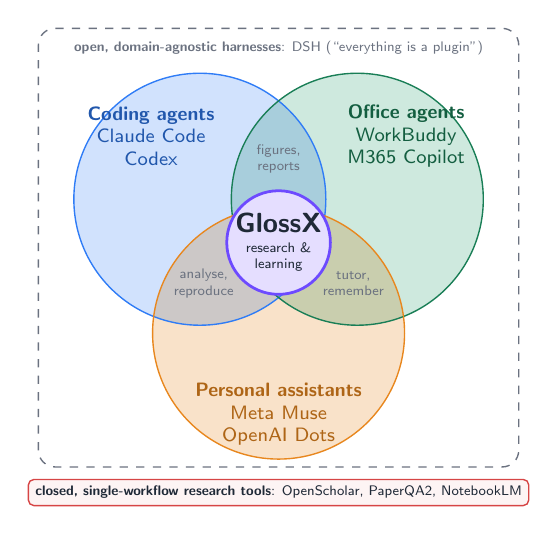
\begin{tikzpicture}[gl]
  % three existing agent categories
  \begin{scope}[blend group=multiply]
    \fill[glblue!22]   (-1.0, 0.55) circle (1.6);
    \fill[glgreen!22]  ( 1.0, 0.55) circle (1.6);
    \fill[glorange!24] ( 0.0,-1.15) circle (1.6);
  \end{scope}
  \draw[glblue]   (-1.0, 0.55) circle (1.6);
  \draw[glgreen!80!black]  ( 1.0, 0.55) circle (1.6);
  \draw[glorange] ( 0.0,-1.15) circle (1.6);

  \node[align=center, text=glblue!70!black] at (-1.62, 1.35)
    {\textbf{Coding agents}\\Claude Code\\Codex};
  \node[align=center, text=glgreen!60!black] at (1.62, 1.35)
    {\textbf{Office agents}\\WorkBuddy\\M365 Copilot};
  \node[align=center, text=glorange!75!black] at (0, -2.18)
    {\textbf{Personal assistants}\\Meta Muse\\OpenAI Dots};

  % what research needs from each overlap
  \node[align=center, font=\sffamily\tiny, text=glgray] at (0, 1.06) {figures,\\reports};
  \node[align=center, font=\sffamily\tiny, text=glgray] at (-0.95,-0.52) {analyse,\\reproduce};
  \node[align=center, font=\sffamily\tiny, text=glgray] at ( 0.95,-0.52) {tutor,\\remember};

  % Gloss at the intersection
  \node[circle, draw=glpurple, line width=1pt, fill=glpurple!18, minimum size=1.22cm,
        align=center, inner sep=0pt] (gloss) at (0, 0.0)
    {\textbf{\normalsize \sysname}\\[-1pt]{\tiny research \&}\\[-2pt]{\tiny learning}};

  % general-purpose open harnesses (domain-agnostic) frame the whole space
  \draw[glgray, dashed, rounded corners=6pt] (-3.05,-2.85) rectangle (3.05, 2.72);
  \node[anchor=north, font=\sffamily\tiny, text=glgray, align=center] at (0, 2.68)
    {\textbf{open, domain-agnostic harnesses}: DSH (``everything is a plugin'')};

  % closed single-workflow research tools
  \node[box, draw=glred, fill=glred!6, font=\sffamily\tiny, align=center, anchor=north]
    (closed) at (0,-3.0)
    {\textbf{closed, single-workflow research tools}: OpenScholar, PaperQA2, NotebookLM};
\end{tikzpicture}
}
  \caption{\textbf{Positioning.} Research needs code (analyse, reproduce), office output (reports, tables) and assistant behaviour (tutoring, memory). \sysname{} sits at their intersection, specialised to scholarly sources, and is open like DSH rather than closed like existing research tools.}
  \label{fig:positioning}
  \vspace{-12pt}
\end{wrapfigure}

Students and researchers switch between a PDF reader, a reference manager, a chatbot, a coding agent and an office suite, and they glue the results together by hand. General agents produce fluent but unverifiable text: on ScholarQABench, GPT-4o fabricates 78--90\% of its citations~\cite{asai2024openscholar}, and a recent survey names verification as the main gap of AI-scientist systems~\cite{ding2026verification}. The tasks are also hard: the best agentic workflow scores only 38.8\% on cross-paper PaperArena questions~\cite{wang2025paperarena}. Figure~\ref{fig:positioning} shows the gap in the market. Coding agents master code but have no notion of sources or evidence. Office agents~\cite{workbuddy2026} and assistants~\cite{muse2026,dots2026} act on apps and errands rather than scholarly corpora. Research tools (OpenScholar~\cite{asai2024openscholar}, PaperQA2~\cite{skarlinski2024paperqa2}, NotebookLM~\cite{notebooklm}) are closed, single-workflow systems. Open harnesses such as DSH~\cite{dsh2026} are domain-agnostic. \sysname{} targets the intersection: a research-and-learning harness that is open like DSH and \emph{delegates} code to existing coding agents instead of re-implementing them.

\textbf{Challenges.}
\textbf{C1 Unification:} Python functions, prompt plugins, SKILL.md skills, MCP servers, CLI coding agents and specialised models must look the same to a single planner.
\textbf{C2 Context:} one paper is 10--30k tokens; multi-paper workflows overflow the context window and multiply cost when text is re-sent.
\textbf{C3 Grounding:} outputs must be verifiable at span level, not merely ``cited''.
\textbf{C4 Openness vs.\ safety:} third-party plugins, code execution, and documents that contain prompt injections.
\textbf{C5 Evaluation:} outputs are open-ended and the API budget is a student budget.

% =====================================================================
\section{Proposed Solution: the \sysname{} Design}
\label{sec:design}

\begin{figure}[t]
  \centering
  \resizebox{\textwidth}{!}{% Figure 2: Gloss Agent architecture -- a small kernel, everything else is a plugin.
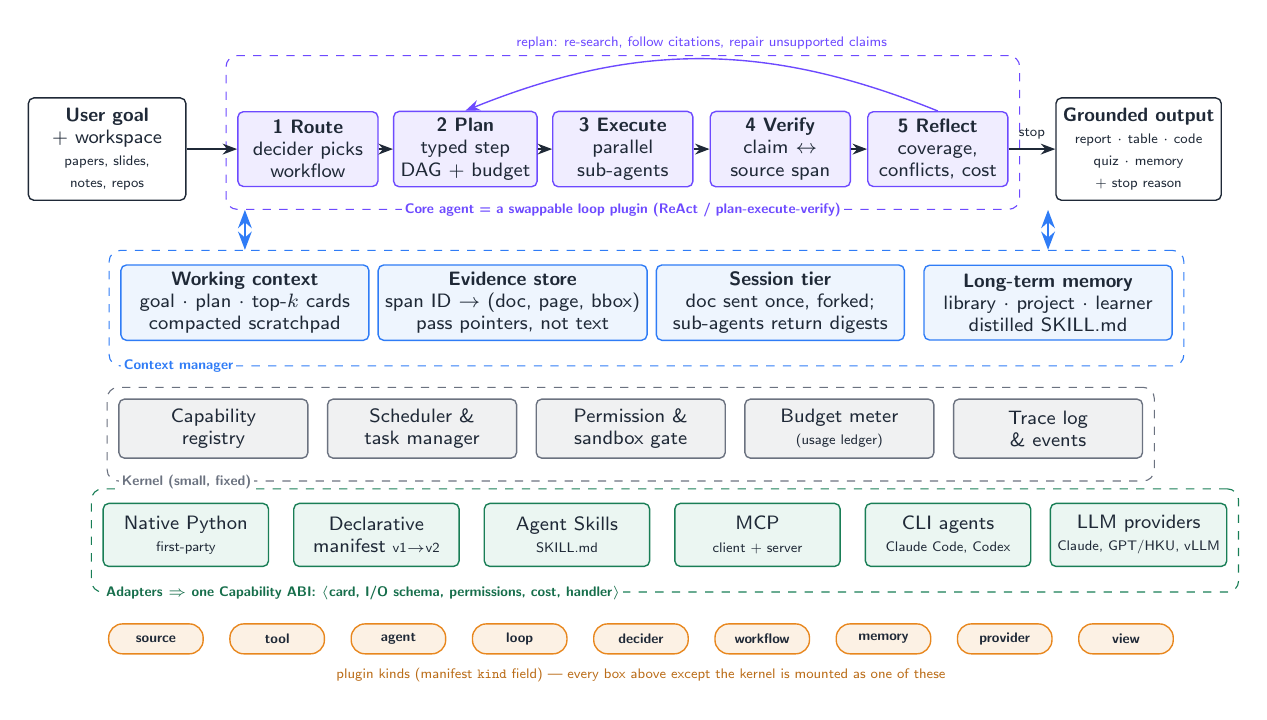
\begin{tikzpicture}[gl]
  % ---------------- core agent loop (itself a loop plugin) ----------------
  \node[io] (in) at (0,6.1) {\textbf{User goal}\\+ workspace\\{\tiny papers, slides,}\\{\tiny notes, repos}};
  \node[gstep] (route)   at (2.55,6.1) {\textbf{1 Route}\\decider picks\\workflow};
  \node[gstep] (plan)    at (4.55,6.1) {\textbf{2 Plan}\\typed step\\DAG + budget};
  \node[gstep] (exec)    at (6.55,6.1) {\textbf{3 Execute}\\parallel\\sub-agents};
  \node[gstep] (verify)  at (8.55,6.1) {\textbf{4 Verify}\\claim $\leftrightarrow$\\source span};
  \node[gstep] (reflect) at (10.55,6.1) {\textbf{5 Reflect}\\coverage,\\conflicts, cost};
  \node[io] (out) at (13.1,6.1) {\textbf{Grounded output}\\{\tiny report $\cdot$ table $\cdot$ code}\\{\tiny quiz $\cdot$ memory}\\{\tiny + stop reason}};
  \draw[flow] (in) -- (route);
  \draw[flow] (route) -- (plan);
  \draw[flow] (plan) -- (exec);
  \draw[flow] (exec) -- (verify);
  \draw[flow] (verify) -- (reflect);
  \draw[flow] (reflect) -- node[above, font=\sffamily\tiny] {stop} (out);
  \draw[flow, glpurple] (reflect.north) to[bend right=22]
     node[above, font=\sffamily\tiny, text=glpurple] {replan: re-search, follow citations, repair unsupported claims} (plan.north);
  \begin{scope}[on background layer]
    \node[frame=glpurple, fit=(route)(reflect), inner ysep=14pt, yshift=6pt] (coreframe) {};
  \end{scope}
  \node[framelabel=glpurple] at (coreframe.south)
    {Core agent = a swappable \textit{loop} plugin (ReAct / plan-execute-verify)};

  % ---------------- context manager ----------------
  \node[ctx] (wc) at (1.75,4.15) {\textbf{Working context}\\goal $\cdot$ plan $\cdot$ top-$k$ cards\\compacted scratchpad};
  \node[ctx] (ev) at (5.15,4.15) {\textbf{Evidence store}\\span ID $\to$ (doc, page, bbox)\\pass pointers, not text};
  \node[ctx] (ss) at (8.55,4.15) {\textbf{Session tier}\\doc sent once, forked;\\sub-agents return digests};
  \node[ctx] (lt) at (11.95,4.15) {\textbf{Long-term memory}\\library $\cdot$ project $\cdot$ learner\\distilled SKILL.md};
  \begin{scope}[on background layer]
    \node[frame=glblue, fit=(wc)(lt), inner ysep=7pt, yshift=-2pt] (ctxframe) {};
  \end{scope}
  \node[framelabel=glblue, anchor=west] at ($(ctxframe.south west)+(0.15,0)$) {Context manager};
  \draw[<->, glblue, line width=0.8pt] (ctxframe.north -| wc) -- (coreframe.south -| wc);
  \draw[<->, glblue, line width=0.8pt] (ctxframe.north -| lt) -- (coreframe.south -| lt);

  % ---------------- kernel ----------------
  \foreach \x/\n/\t in {1.35/k1/{Capability\\registry}, 4.0/k2/{Scheduler \&\\task manager},
                        6.65/k3/{Permission \&\\sandbox gate}, 9.3/k4/{Budget meter\\{\tiny (usage ledger)}},
                        11.95/k5/{Trace log\\\& events}}
    \node[kern] (\n) at (\x,2.55) {\t};
  \begin{scope}[on background layer]
    \node[frame=glgray, fit=(k1)(k5), inner ysep=6pt, yshift=-2pt] (kframe) {};
  \end{scope}
  \node[framelabel=glgray, anchor=west] at ($(kframe.south west)+(0.15,0)$) {Kernel (small, fixed)};

  % ---------------- adapters ----------------
  \foreach \i/\t in {0/{Native Python\\{\tiny first-party}}, 1/{Declarative\\manifest {\tiny v1$\to$v2}},
                     2/{Agent Skills\\{\tiny SKILL.md}}, 3/{MCP\\{\tiny client + server}},
                     4/{CLI agents\\{\tiny Claude Code, Codex}}, 5/{LLM providers\\{\tiny Claude, GPT/HKU, vLLM}}}
    \node[adp] (a\i) at ({1.0+\i*2.42},1.2) {\t};
  \begin{scope}[on background layer]
    \node[frame=glgreen!80!black, fit=(a0)(a5), inner ysep=7pt, yshift=-2pt] (aframe) {};
  \end{scope}
  \node[framelabel=glgreen!70!black, anchor=west] at ($(aframe.south west)+(0.15,0)$)
    {Adapters $\Rightarrow$ one Capability ABI: $\langle$card, I/O schema, permissions, cost, handler$\rangle$};

  % ---------------- plugin kinds ----------------
  \foreach \i/\t in {0/source,1/tool,2/agent,3/loop,4/decider,5/workflow,6/memory,7/provider,8/view}
    \node[chip] (c\i) at ({0.62+\i*1.54},-0.12) {\t};
  \node[font=\sffamily\tiny, text=glorange!80!black, anchor=north] at (6.78,-0.37)
    {plugin kinds (manifest \texttt{kind} field) --- every box above except the kernel is mounted as one of these};
\end{tikzpicture}
}
  \caption{\textbf{\sysname{} architecture.} A fixed kernel; everything else, including the core loop, is a plugin compiled by an adapter into one Capability ABI. The core agent routes, plans, executes, verifies and reflects, and the context manager keeps full texts out of the planner's window.}
  \label{fig:arch}
  \vspace{-6pt}
\end{figure}

\subsection{Everything is a plugin: one Capability ABI (C1)}
The kernel is deliberately small: a capability registry, a scheduler (\gloss{}'s existing task manager, which already supports unbounded concurrency, cancellation and progress), a permission and sandbox gate, a budget meter (the existing usage ledger), and a trace log (Fig.~\ref{fig:arch}). Everything else is a plugin with a manifest (\texttt{api\_version: 2}, \texttt{kind} $\in$ \{source, tool, agent, loop, decider, workflow, memory, provider, view\}; example in App.~\ref{app:manifest}). Adapters compile every plugin into a \emph{Capability} $\langle$card, I/O schema, requirements, permissions, cost and side-effect hints, handler$\rangle$. The \emph{card} is a description of at most 100 tokens that the planner sees; the full schema and instructions are loaded only when the capability is selected (progressive disclosure, as in Agent Skills~\cite{agentskills2025}). There are five adapters:
(i)~\emph{native Python} for trusted first-party plugins;
(ii)~\emph{declarative manifests}, so all nine v1 plugins upgrade automatically into tools whose prompt becomes the handler;
(iii)~\emph{SKILL.md} skills from Claude, Codex or agentskills.io;
(iv)~\emph{MCP}~\cite{mcp2024}, where \sysname{} is both a client (e.g., Zotero and arXiv servers become tools) and a server (exposing the library, spans and annotations to external agents);
(v)~\emph{CLI agents}, where Claude Code and Codex become sandboxed \texttt{delegate} tools with their tools enabled in a per-project workspace.
Because the loop and the decider are plugins too, a ReAct loop~\cite{yao2023react}, a plan--execute--verify loop, or a Jev-backed decider~\cite{jev2026} can be swapped in without touching the kernel.

\subsection{How the core agent invokes plugins}
\textbf{(1) Route.} A decider maps the goal and workspace to a workflow plugin, or to the generic loop, using capability cards (BM25 retrieves the top-$k$ cards when the registry is large).
\textbf{(2) Plan.} A planner emits a typed step graph (DAG). Each step names a capability, its inputs (span IDs or artifacts), a success criterion and a budget.
\textbf{(3) Execute.} The loop dispatches ready steps, and independent steps (e.g., one reader per paper) run in parallel as kernel tasks. Every call passes the permission gate and budget meter and is traced.
\textbf{(4) Verify.} A verifier splits outputs into atomic claims and retrieves candidate spans; a decider labels each claim supported, partial or unsupported with a confidence. Unsupported claims are repaired or removed.
\textbf{(5) Reflect.} Using sub-question coverage, conflicts and remaining budget, the loop replans (re-search, follow citations, read further) or stops with an explicit reason: goal met, budget exhausted, no progress for $k$ rounds, or approval needed~\cite{shinn2023reflexion}. Tool failures, timeouts and offline sources become observations, so the agent retries with an alternative capability (e.g., arXiv $\to$ Semantic Scholar $\to$ local library).

\subsection{Context management: pass pointers, not text (C2, C3)}
\textbf{Working context} holds only the goal, the plan, the current step, the top-$k$ cards and a scratchpad. Older steps are compacted into summaries that keep their IDs.
\textbf{Evidence store:} source plugins normalise PDFs, \LaTeX{}, Markdown, slides and web pages into \emph{spans} with stable IDs $\to$ (doc, page, bbox). Agents exchange span IDs, and text is materialised under a token budget only when it is needed. The same IDs make every final claim clickable back to its location in the reader.
\textbf{Session tier:} \gloss{}'s shared paper session sends a document once per provider session, and sub-agents fork it. Each reader works in an isolated context with only its document and returns a schema-bound digest (map--reduce), so the orchestrator never holds full texts.
\textbf{Long-term memory} covers the library, project memory (findings, decisions, preferences), a learner model, and SKILL.md files distilled from successful traces for reuse in later tasks.

\subsection{Openness vs.\ safety (C4)}
Plugins have trust tiers. First-party plugins may contain code. Third-party plugins stay declarative compositions of existing capabilities, which keeps \gloss{}'s rule of never executing downloaded code. Code runs only through sandboxed delegates, under approval and a budget. MCP servers get scoped permissions. Document text and tool outputs are tagged as untrusted data and can never issue tool calls.

\subsection{Plugin roadmap}
Table~\ref{tab:plugins} lists the plugins we plan to build, the agentic behaviour each one exercises, and how each will be evaluated. Core rows are committed; stretch rows depend on time and API access.
Together they cover every agentic capability in the project brief: planning (Plan), tool selection (Route over capability cards), multi-step execution (Execute), iterative verification (Verify), external environments (MCP, web search, coding agents), memory (the context tiers), reflection and error recovery (Reflect), and multi-agent collaboration (the reader swarm and the planner, reader, verifier and writer roles).

\begin{table}[t]
  \caption{\textbf{Planned plugins}, the agentic behaviour each exercises, and its evaluation. Dataset details are in App.~\ref{app:bench}.}
  \label{tab:plugins}
  \centering
  \scriptsize
  \setlength{\tabcolsep}{3pt}
  \renewcommand{\arraystretch}{1.08}
  \begin{tabularx}{\textwidth}{@{}>{\raggedright\arraybackslash}p{2.75cm}>{\raggedright\arraybackslash}X>{\raggedright\arraybackslash}p{4.6cm}c@{}}
    \toprule
    \textbf{Plugin} (\textit{kind}) & \textbf{Agentic behaviour} & \textbf{Benchmark / metric} & \textbf{Tier} \\
    \midrule
    Literature review (\textit{workflow}) & plan sub-questions, search, parallel readers, verify, re-search until coverage & AutoResearchBench~\cite{xiong2026autoresearchbench}, LitSearch~\cite{ajith2024litsearch}: Recall@$k$, nDCG & core \\
    Cross-paper QA (\textit{workflow}) & select tools across papers, tables and figures; multi-hop & PaperArena~\cite{wang2025paperarena} acc.; QASPER~\cite{dasigi2021qasper} F1, evidence recall & core \\
    Claim verifier (\textit{agent+decider}) & claim decomposition, span retrieval, self-correction & SciFact~\cite{wadden2020scifact} acc./F1, ECE; ScholarQABench citation P/R & core \\
    Reproduction (\textit{workflow+delegate}) & read method $\to$ plan $\to$ code via Claude Code/Codex $\to$ run $\to$ compare & PaperBench Code-Dev~\cite{starace2025paperbench} rubric (3--5 papers) & core \\
    Study \& tutor (\textit{workflow+memory}) & slides/notes $\to$ concept map $\to$ quiz $\to$ adapt to the learner model & TutorBench~\cite{srinivasa2025tutorbench} rubric subset; course slides, human rating & core \\
    New sources (\textit{source}) & Markdown, slides, web, \LaTeX{} $\to$ span store & QA parity of PDF vs.\ other formats; parse fidelity & core \\
    MCP bridge (\textit{tool/provider}) & Zotero/arXiv tools in; \sysname{} exposed out & routing success; interop with Claude Code/Codex & core \\
    Comparison tables (\textit{agent}) & multi-paper aspect extraction & ArxivDIGESTables~\cite{newman2024arxivdigestables} (AstaBench~\cite{bragg2025astabench}) & stretch \\
    Skill distillation (\textit{memory}) & write reusable SKILL.md from successful traces & success and token change on re-runs & stretch \\
    Jev decider (\textit{decider}) & typed, calibrated routing and verification & accuracy, ECE, latency, cost vs.\ LLM decider & stretch \\
    Research radar (\textit{loop}) & scheduled arXiv watch against project memory & precision@10 vs.\ member labels & stretch \\
    \bottomrule
  \end{tabularx}
  \vspace{-8pt}
\end{table}

% =====================================================================
\section{Experimental Datasets and Evaluation Plan}
\label{sec:eval}

\textbf{Data sources.}
(a)~The public benchmarks in Table~\ref{tab:plugins}, subsampled to 50--100 items each to fit the API budget.
(b)~\emph{\sysname{}-Route-100}: 100 heterogeneous research and study requests (find, compare, verify, reproduce, learn), each labelled with its gold workflow and capability set, written and cross-checked by group members.
(c)~Slides and notes from this course, for the study workflow.
(d)~A fault-injection suite: offline network, provider timeouts, malformed PDFs, failing plugins, and instructions injected into documents.

\textbf{Metrics.}
\emph{Quality:} each benchmark's native metric (Recall@$k$/nDCG, accuracy/F1, rubric score) plus citation precision/recall and the span-level support rate.
\emph{Reliability:} task success, recovery rate under faults, and variance over 3 runs.
\emph{Efficiency:} latency, tokens and cost from the usage ledger, and the number of tool calls.
\emph{Extensibility:} manifest/code lines needed to add a workflow, and the size of the kernel diff (target: none).

\textbf{Baselines and ablations.}
B0 is \gloss{} v1.0.2's single-prompt features, B1 is standard RAG, and B2 is \sysname{}; published scores are given for reference.
Ablations remove the verifier or reflection, compare a single agent with a reader swarm, vary the loop budget (1/2/3 rounds), compare full context with pointers plus a shared session, compare an LLM decider with a Jev decider, and swap model backends (HKU GPT models, Claude, Codex, and an open model on vLLM).
Rubric judgements use an LLM judge, and humans spot-check 20\% of them (Cohen's $\kappa$). Failures are categorised as retrieval miss, wrong tool, unsupported claim, non-termination or budget overrun.

\textbf{Success criteria.} B2 beats B0 and B1 on PaperArena accuracy and citation precision at comparable cost; routing accuracy on \sysname{}-Route-100 is at least 90\%; the last three workflows are added without kernel changes; and the system degrades gracefully in every fault scenario.

% =====================================================================
\bibliographystyle{plainnat}
{\small \bibliography{references}}

\newpage
\appendix
\raggedbottom

\section{Example plugin manifest (v2)}
\label{app:manifest}
Version-1 manifests remain valid; \texttt{kind}, \texttt{capability} and \texttt{steps} are the v2 additions. A workflow is a declarative composition of other capabilities, so third-party authors never ship code.
\begin{lstlisting}
{
  "api_version": 2,
  "id": "glossx.literature-review",
  "kind": "workflow",
  "name": "Literature Review",
  "permissions": ["library:read", "search:web", "ai:complete"],
  "capability": {
    "card": "Answer a research question with a cited review: plan sub-questions, search, read papers in parallel, verify every claim, and re-search until coverage is met.",
    "input":  {"question": "string", "max_papers": "integer"},
    "output": {"report": "markdown", "claims": "claim[] with span_ids"}
  },
  "steps": [
    {"id": "plan",    "use": "agent:planner"},
    {"id": "search",  "use": "tool:scholar.search", "fallback": ["mcp:zotero.search", "tool:library.search"]},
    {"id": "screen",  "use": "decider:relevance"},
    {"id": "read",    "use": "agent:reader", "map_over": "screen.accepted", "context": "shared_session"},
    {"id": "verify",  "use": "agent:verifier"},
    {"id": "write",   "use": "agent:writer"}
  ],
  "loop": {"use": "loop:plan-execute-verify", "stop": {"coverage": 0.8, "max_rounds": 3, "max_usd": 0.5}},
  "agent": {"name": "Review Scout", "icon": "telescope"}
}
\end{lstlisting}

\section{Workflow example: literature review}
\begin{figure}[H]
  \centering
  \resizebox{\textwidth}{!}{% Figure 3 (appendix): the literature-review workflow plugin, step by step.
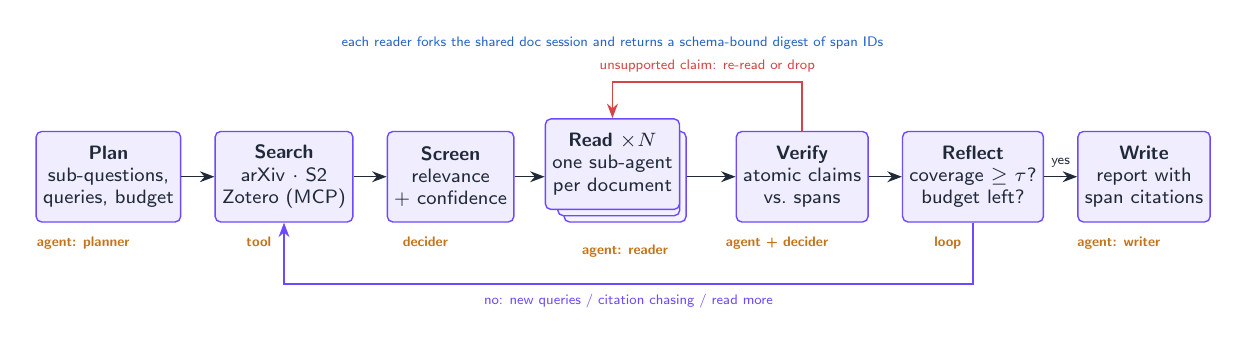
\begin{tikzpicture}[gl, node distance=0.42cm]
  \tikzset{w/.style={gstep, minimum width=1.55cm, minimum height=1.15cm},
           kind/.style={font=\sffamily\tiny\bfseries, text=glorange!85!black}}
  \node[w] (plan) {\textbf{Plan}\\sub-questions,\\queries, budget};
  \node[w, right=of plan] (search) {\textbf{Search}\\arXiv $\cdot$ S2\\Zotero (MCP)};
  \node[w, right=of search] (screen) {\textbf{Screen}\\relevance\\+ confidence};
  % reader swarm as stacked boxes
  \node[w, right=0.62cm of screen, fill=glpurple!6] (r3) {};
  \node[w, fill=glpurple!8] (r2) at ($(r3)+(-0.08,0.08)$) {};
  \node[w] (read) at ($(r3)+(-0.16,0.16)$) {\textbf{Read} $\times N$\\one sub-agent\\per document};
  \node[w, right=0.62cm of r3] (verify) {\textbf{Verify}\\atomic claims\\vs.\ spans};
  \node[w, right=of verify] (reflect) {\textbf{Reflect}\\coverage $\geq\tau$?\\budget left?};
  \node[w, right=of reflect] (write) {\textbf{Write}\\report with\\span citations};

  \draw[flow] (plan) -- (search);
  \draw[flow] (search) -- (screen);
  \draw[flow] (screen) -- (read.west |- screen);
  \draw[flow] (r3) -- (verify);
  \draw[flow] (verify) -- (reflect);
  \draw[flow] (reflect) -- node[above, font=\sffamily\tiny]{yes} (write);
  \draw[flow, glpurple] (reflect.south) -- ++(0,-0.78) -| node[pos=0.25, below, font=\sffamily\tiny, text=glpurple]
     {no: new queries / citation chasing / read more} (search.south);
  \draw[flow, glred] (verify.north) -- ++(0,0.62) -| node[pos=0.25, above, font=\sffamily\tiny, text=glred]
     {unsupported claim: re-read or drop} (read.north);

  % plugin kinds under each step
  \foreach \n/\k in {plan/agent: planner, search/tool, screen/decider, verify/agent + decider,
                     reflect/loop, write/agent: writer}
    \node[kind, below=0.06cm of \n, xshift=-0.32cm] {\k};
  \node[kind, below=0.16cm of r3] {agent: reader};

  % context annotations
  \node[font=\sffamily\tiny, text=glblue!80!black, align=center, above=0.75cm of read]
    {each reader forks the shared doc session and returns a schema-bound digest of span IDs};
\end{tikzpicture}
}
  \caption{The literature-review workflow plugin. Each step is a capability of the indicated kind. The reflect step loops back to search when coverage is below $\tau$, and the verifier sends unsupported claims back to the readers.}
  \label{fig:workflow}
\end{figure}

\section{Benchmark details}
\label{app:bench}
\begin{table}[H]
  \centering
  \scriptsize
  \setlength{\tabcolsep}{3pt}
  \begin{tabularx}{\textwidth}{@{}>{\raggedright\arraybackslash}p{2.6cm}>{\raggedright\arraybackslash}p{3.6cm}>{\raggedright\arraybackslash}Xc@{}}
    \toprule
    \textbf{Benchmark} & \textbf{Content} & \textbf{Why it fits \sysname{}} & \textbf{Planned $n$} \\
    \midrule
    PaperArena~\cite{wang2025paperarena} & 784 tool-augmented cross-paper QA pairs (AI papers) & multi-step, multi-paper tool use; best published workflow 38.8\% & 100 \\
    AutoResearchBench~\cite{xiong2026autoresearchbench} & expert-verified literature discovery; Deep and Wide research tasks & tests the search--reflect loop and coverage stopping & 50 \\
    LitSearch~\cite{ajith2024litsearch} & 597 literature-search queries (ML/NLP) & cheap, stable retrieval recall & 100 \\
    ScholarQABench~\cite{asai2024openscholar} & 2{,}967 expert queries, 208 long-form answers & citation precision/recall of synthesised answers & 50 \\
    QASPER~\cite{dasigi2021qasper} & QA over NLP papers with evidence annotations & span grounding of single-paper answers & 100 \\
    SciFact~\cite{wadden2020scifact} & scientific claim verification & verifier and decider accuracy and calibration & 100 \\
    PaperBench Code-Dev~\cite{starace2025paperbench} & rubric-graded code development for ICML papers, no GPU needed & delegation to coding agents & 3--5 \\
    TutorBench~\cite{srinivasa2025tutorbench} & 1{,}490 rubric-graded tutoring samples & explanation, feedback and hint quality & 60 \\
    ArxivDIGESTables~\cite{newman2024arxivdigestables} & literature-review tables (AstaBench subset) & multi-paper aspect extraction & 30 \\
    \sysname{}-Route-100 (ours) & 100 heterogeneous requests with gold workflow/capabilities & routing and tool selection across plugins & 100 \\
    \bottomrule
  \end{tabularx}
\end{table}

\section{Timeline and division of labour}
\begin{table}[H]
  \centering
  \scriptsize
  \begin{tabularx}{\textwidth}{@{}p{2.3cm}Xp{3.2cm}@{}}
    \toprule
    \textbf{Weeks (2026)} & \textbf{Milestone} & \textbf{Owner(s)} \\
    \midrule
    10 Oct -- 19 Oct & kernel, Capability ABI, v1$\to$v2 adapter, trace log & Cai Jiechao (lead), Cai Zhuorui \\
    20 Oct -- 2 Nov & core loop, router/planner/verifier, context manager; MCP/Skills/CLI adapters & Cai Jiechao, Cai Zhuorui, Sun Zhiwei \\
    3 Nov -- 16 Nov & literature review, cross-paper QA, reproduction and tutor workflows; new sources & Cai Zhuorui, Sun Zhiwei, Zhang Guanyi \\
    10 Nov -- 23 Nov & benchmark harness, \sysname{}-Route-100, fault injection, ablations & Zhang Guanyi (eval lead), all \\
    24 Nov -- end & stretch plugins, report, presentation demo & all \\
    \bottomrule
  \end{tabularx}
\end{table}

\section{Risks and limitations}
\begin{itemize}
  \item \textbf{API access and budget.} Jev access is uncertain; the decider ABI falls back to a small LLM with a JSON schema. Benchmarks are subsampled, and costs are tracked per run.
  \item \textbf{Judge bias and contamination.} LLM judges are spot-checked by humans, and older benchmarks may appear in model training data, so we also include 2026 benchmarks and our own tasks.
  \item \textbf{Coding-agent cost and safety.} Reproduction runs are sandboxed, capped by budget and limited to a few papers.
  \item \textbf{Scope.} Core rows of Table~\ref{tab:plugins} are prioritised; stretch plugins are explicitly optional.
\end{itemize}

\end{document}
